% !TEX TS-program = xelatex
% !BIB TS-program = bibtex
\documentclass[12pt,letterpaper]{article}
\usepackage{style/dsc180reportstyle} % import dsc180reportstyle.sty
\usepackage{float} % for [H] figure placement

%%%%%%%%%%%%%%%%%%%%%%%%%%%%%%%%%%%%%%%%%%%%%%%%%%%%%%%%
%%%% Title and Authors
%%%%%%%%%%%%%%%%%%%%%%%%%%%%%%%%%%%%%%%%%%%%%%%%%%%%%%%%

\title{DSC Capstone Q2 Report}

\author{Jevan Chahal\\
  {\tt j2chahal@ucsd.edu} \\\And
  Hillary Change \\
  {\tt hic001@ucsd.edu} \\\And
  Kurumi Kaneko \\
  {\tt kskaneko@ucsd.edu} \\\And
  Kevin Wong \\
  {\tt kew024@ucsd.edu} \\\And
  Brian Duke \\
  {\tt brian.duke@prismdata.com} \\\And
  Kyle Nero \\
  {\tt kyle.nero@prismdata.com} \\}

\begin{document}
\maketitle

%%%%%%%%%%%%%%%%%%%%%%%%%%%%%%%%%%%%%%%%%%%%%%%%%%%%%%%%
%%%% Abstract and Links
%%%%%%%%%%%%%%%%%%%%%%%%%%%%%%%%%%%%%%%%%%%%%%%%%%%%%%%%

\begin{abstract}
    \textcolor{black}{
    The process of capturing what makes a creditor trustworthy or not is especially vital within the confines of bank data, due to the guidelines and ethics of what makes this data usable. Although the quantity of the data is massive, there are only a few available features that are explicitly useful in the confines of machine learning, which calls into question how we should measure customer's trustworthiness towards their creditors. Our methodology details the process of refining bank data into categories using Natural Language Processing, assessing individual's income based on bank data alone, and also measuring their credit worthiness both accurately and efficiently. 
    }
\end{abstract}

\begin{center}
Code: \url{https://github.com/hillarychang/dsc180b-capstone-q2}
\end{center}

\maketoc
\clearpage

%%%%%%%%%%%%%%%%%%%%%%%%%%%%%%%%%%%%%%%%%%%%%%%%%%%%%%%%
%%%% Main Contents
%%%%%%%%%%%%%%%%%%%%%%%%%%%%%%%%%%%%%%%%%%%%%%%%%%%%%%%%
\section{Introduction}

Access to credit is crucial for financial stability, yet traditional credit scoring models often exclude individuals with limited credit history. The "Cash Score" project aims to address this issue by utilizing transaction data to evaluate financial behaviors rather than just historical credit data. Our goal is to provide a more equitable scoring system that benefits both consumers and financial institutions.

\subsection{Data Description}
We utilized multiple datasets that provide consumer transaction details, account balances, and delinquency indicators:
\begin{itemize}
    \item \textbf{q2-ucsd-consDF.pqt}: Contains consumer attributes like \texttt{consumer\_id}, \texttt{credit\_score}, and \texttt{DQ\_target} (delinquency indicator).
    \item \textbf{q2-ucsd-acctDF.pqt}: Includes account-level data such as \texttt{consumer\_id}, \texttt{account\_id}, \texttt{balance\_date}, and \texttt{balance}.
    \item \textbf{q2-ucsd-trxnDF.pqt}: Captures transactional details including \texttt{category}, \texttt{amount}, \texttt{credit\_or\_debit}, and \texttt{posted\_date}.
    \item \textbf{categories.csv}: Maps transaction categories like Rent, Groceries, and Entertainment.
\end{itemize}

\begin{figure}[H]
    \centering
    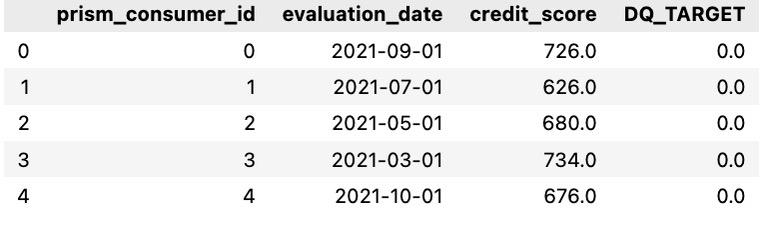
\includegraphics[width=\textwidth]{figure/consumer_df.jpeg}
    \caption{First few columns of the consumer dataset, including consumer ID, evaluation date, credit score, and delinquency target.}
    \label{fig:consumer_df}
\end{figure}

\begin{figure}[H]
    \centering
    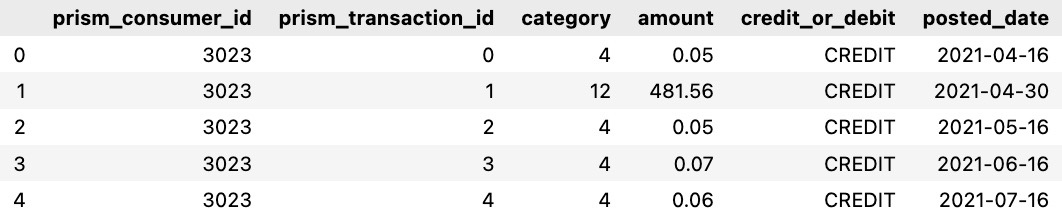
\includegraphics[width=\textwidth]{figure/transactions_df.jpeg}
    \caption{First few columns of the transactions dataset, showing transaction IDs, categories, amounts, and whether they were credit or debit.}
    \label{fig:transactions_df}
\end{figure}

\begin{figure}[H]
    \centering
    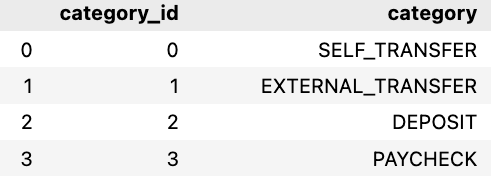
\includegraphics[width=0.7\textwidth]{figure/categories_df.png}
    \caption{First few columns of the transaction categories dataset, mapping category IDs to their corresponding descriptions.}
    \label{fig:categories_df}
\end{figure}


\begin{figure}[H]
    \centering
    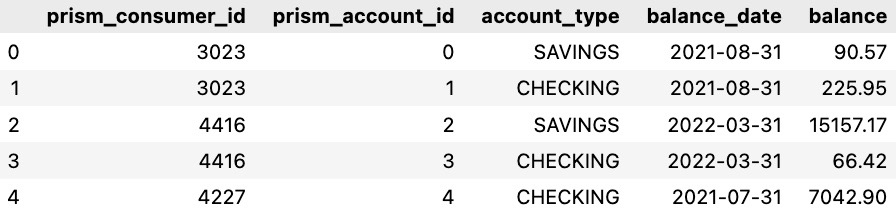
\includegraphics[width=\textwidth]{figure/accounts_df.jpeg}
    \caption{First few columns of the accounts dataset, including account IDs, account types, balance dates, and balances.}
    \label{fig:accounts_df}
\end{figure}

\begin{figure}[H]
    \centering
    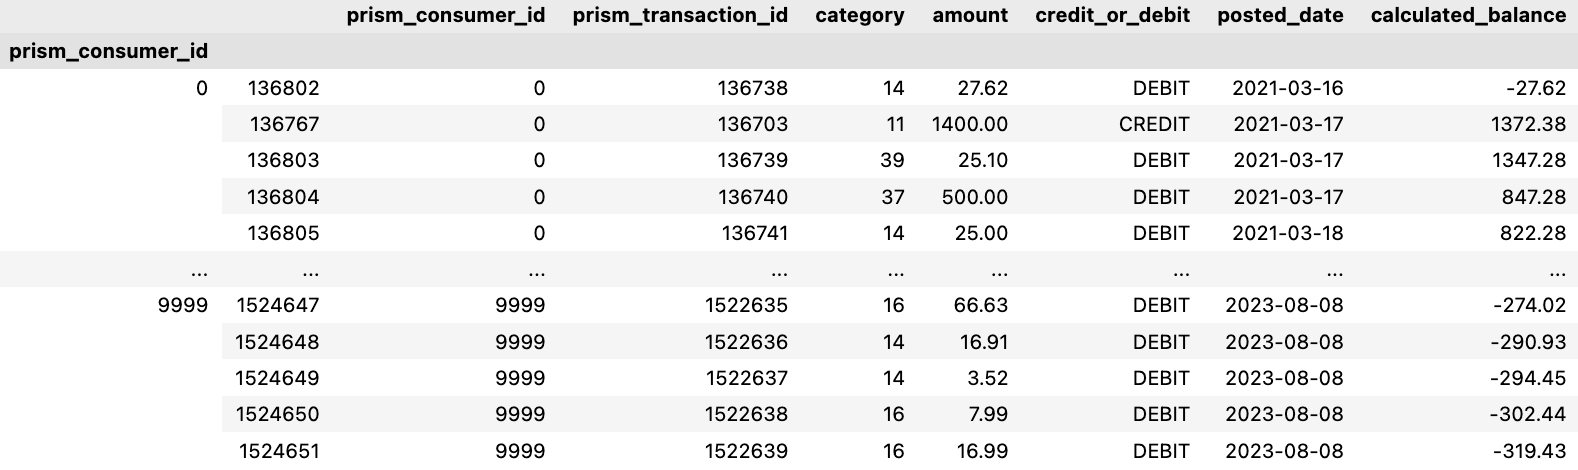
\includegraphics[width=\textwidth]{figure/final_transaction_balance.png}
    \caption{Dataframe showing all user transactions along with their account balances. Credit transactions (inflows) are added while debit transactions (outflows) are subtracted.}
    \label{fig:final_transaction_balance}
\end{figure}


\section{Methodology}

\subsection{Exploratory Data Analysis}
\begin{itemize}
    \item Identified differences in transaction patterns between delinquent and non-delinquent consumers.
    \item Examined seasonal trends, payday effects, and spending fluctuations.
    \item Analyzed the impact of account fees, buy-now-pay-later (BNPL) transactions, and overdrafts.
\end{itemize}

\subsection{Balance Trends for Delinquent vs. Non-Delinquent Consumers}

\begin{figure}[H]
    \centering
    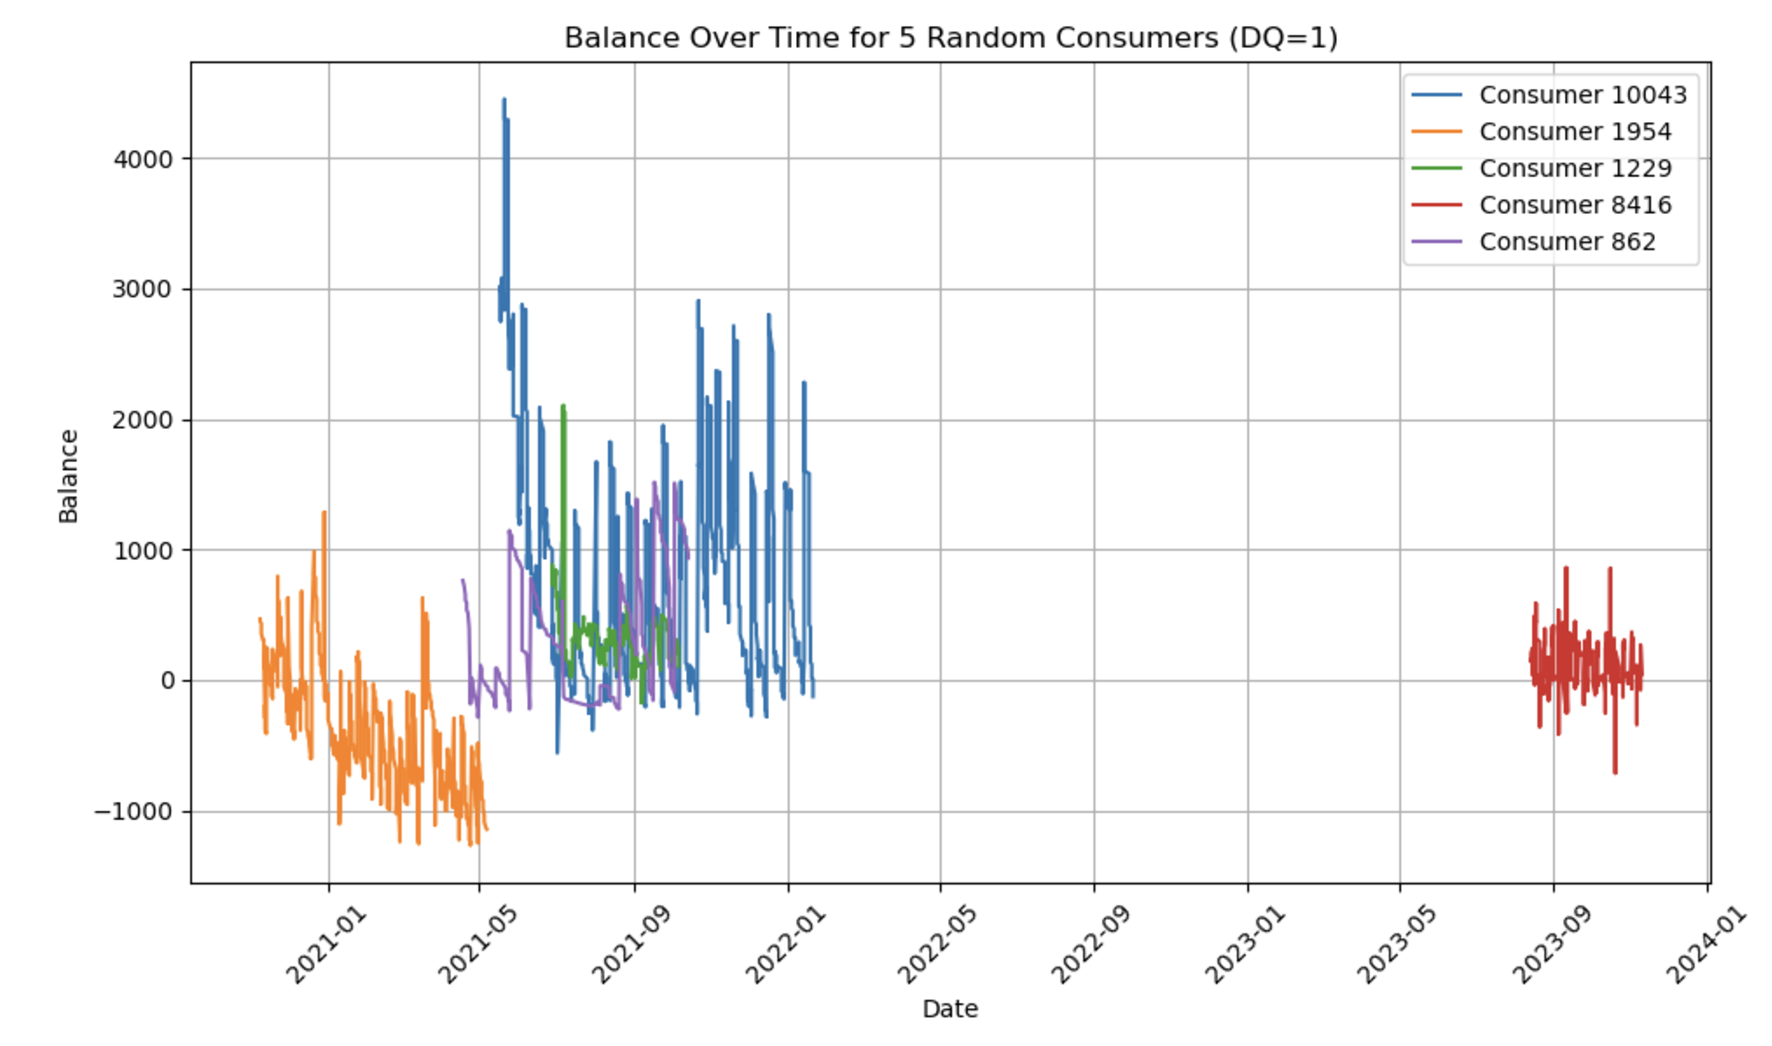
\includegraphics[width=0.7\textwidth]{figure/balance_delinquent.png}
    \caption{Balance trends over time for five randomly selected delinquent consumers. The plot illustrates fluctuations and frequent occurrences of negative balances, highlighting financial instability.}
    \label{fig:balance_delinquent}
\end{figure}

\begin{figure}[H]
    \centering
    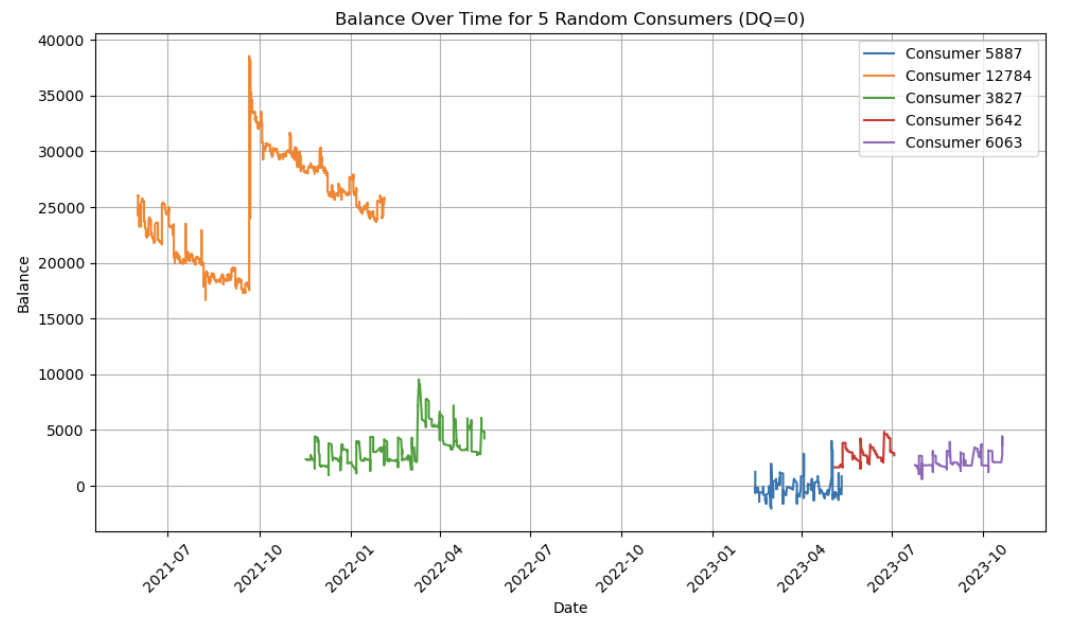
\includegraphics[width=0.7\textwidth]{figure/balance_non_delinquent.png}
    \caption{Balance trends over time for five randomly selected non-delinquent consumers. Compared to delinquent consumers, these users maintain more stable balances with fewer instances of overdrafts.}
    \label{fig:balance_non_delinquent}
\end{figure}

\begin{figure}[H]
    \centering
    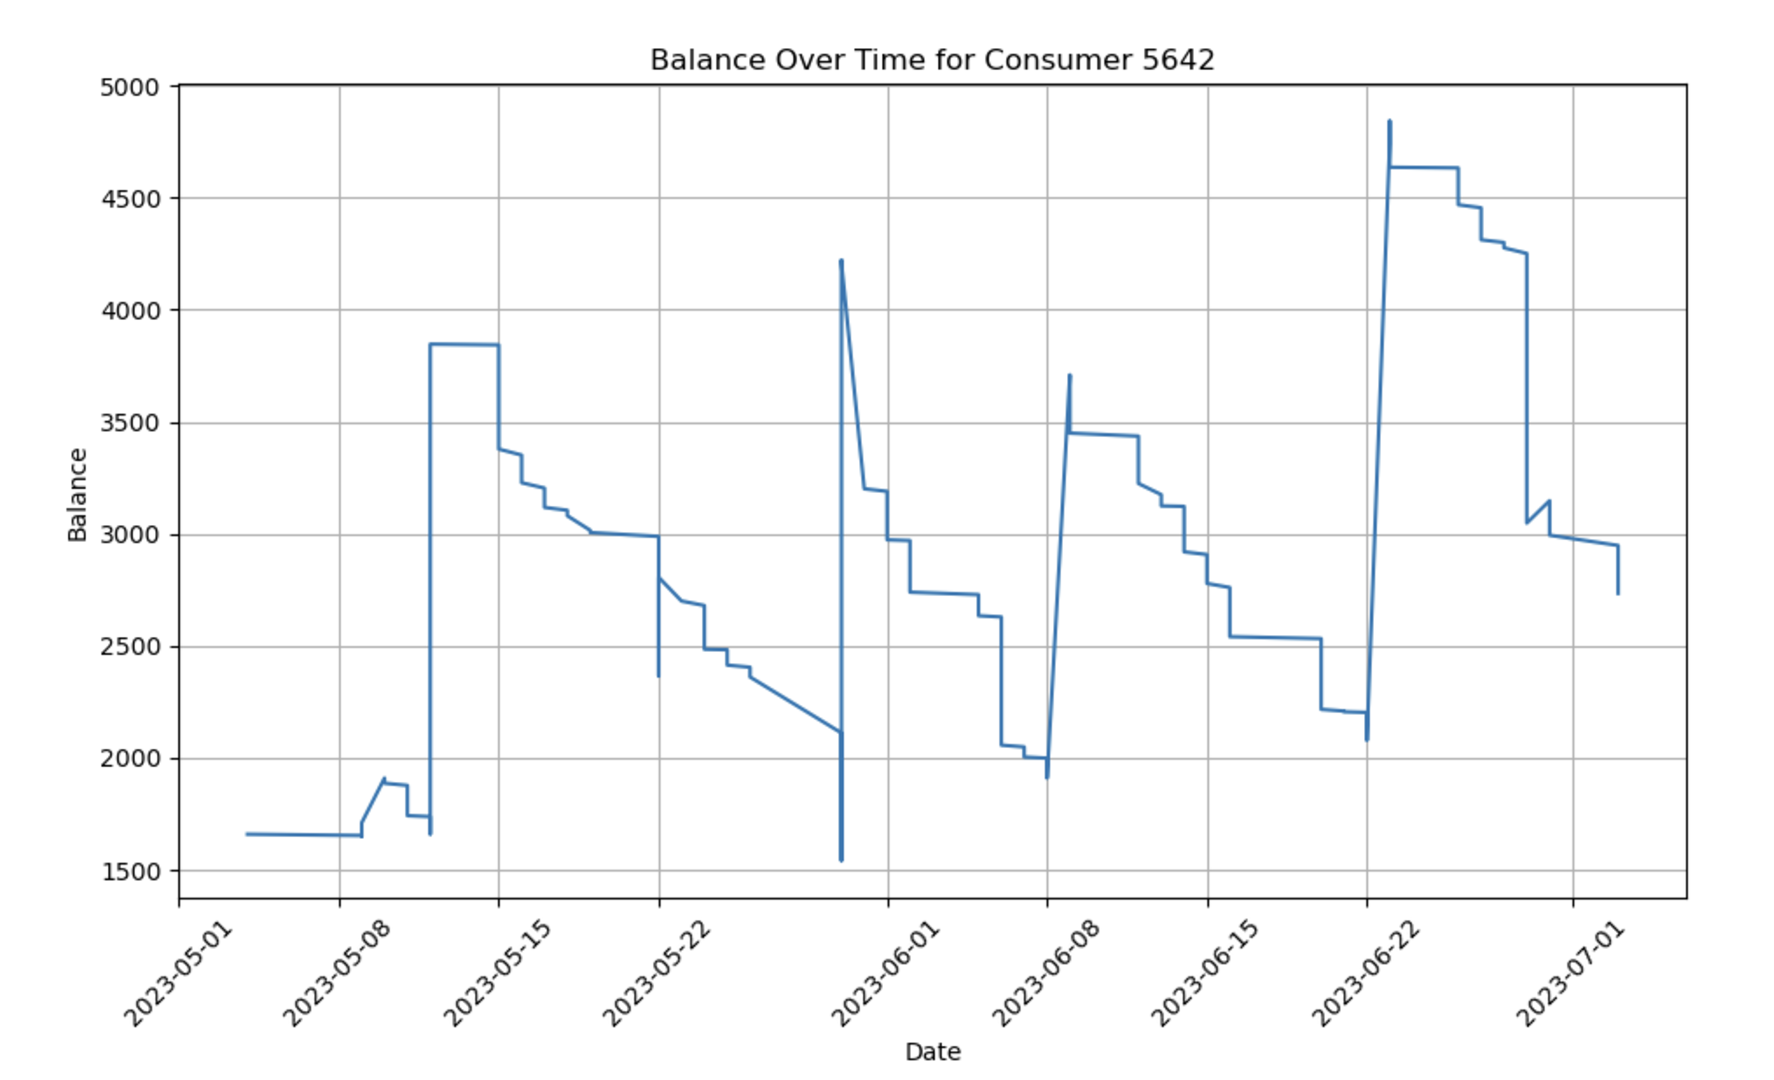
\includegraphics[width=0.7\textwidth]{figure/balance_single_non_delinquent.png}
    \caption{Balance over time for a single non-delinquent consumer. The balance exhibits periodic fluctuations, potentially due to income deposits and spending patterns, but remains above zero for the majority of the observed period.}
    \label{fig:balance_single_non_delinquent}
\end{figure}

\begin{figure}[H]
    \centering
    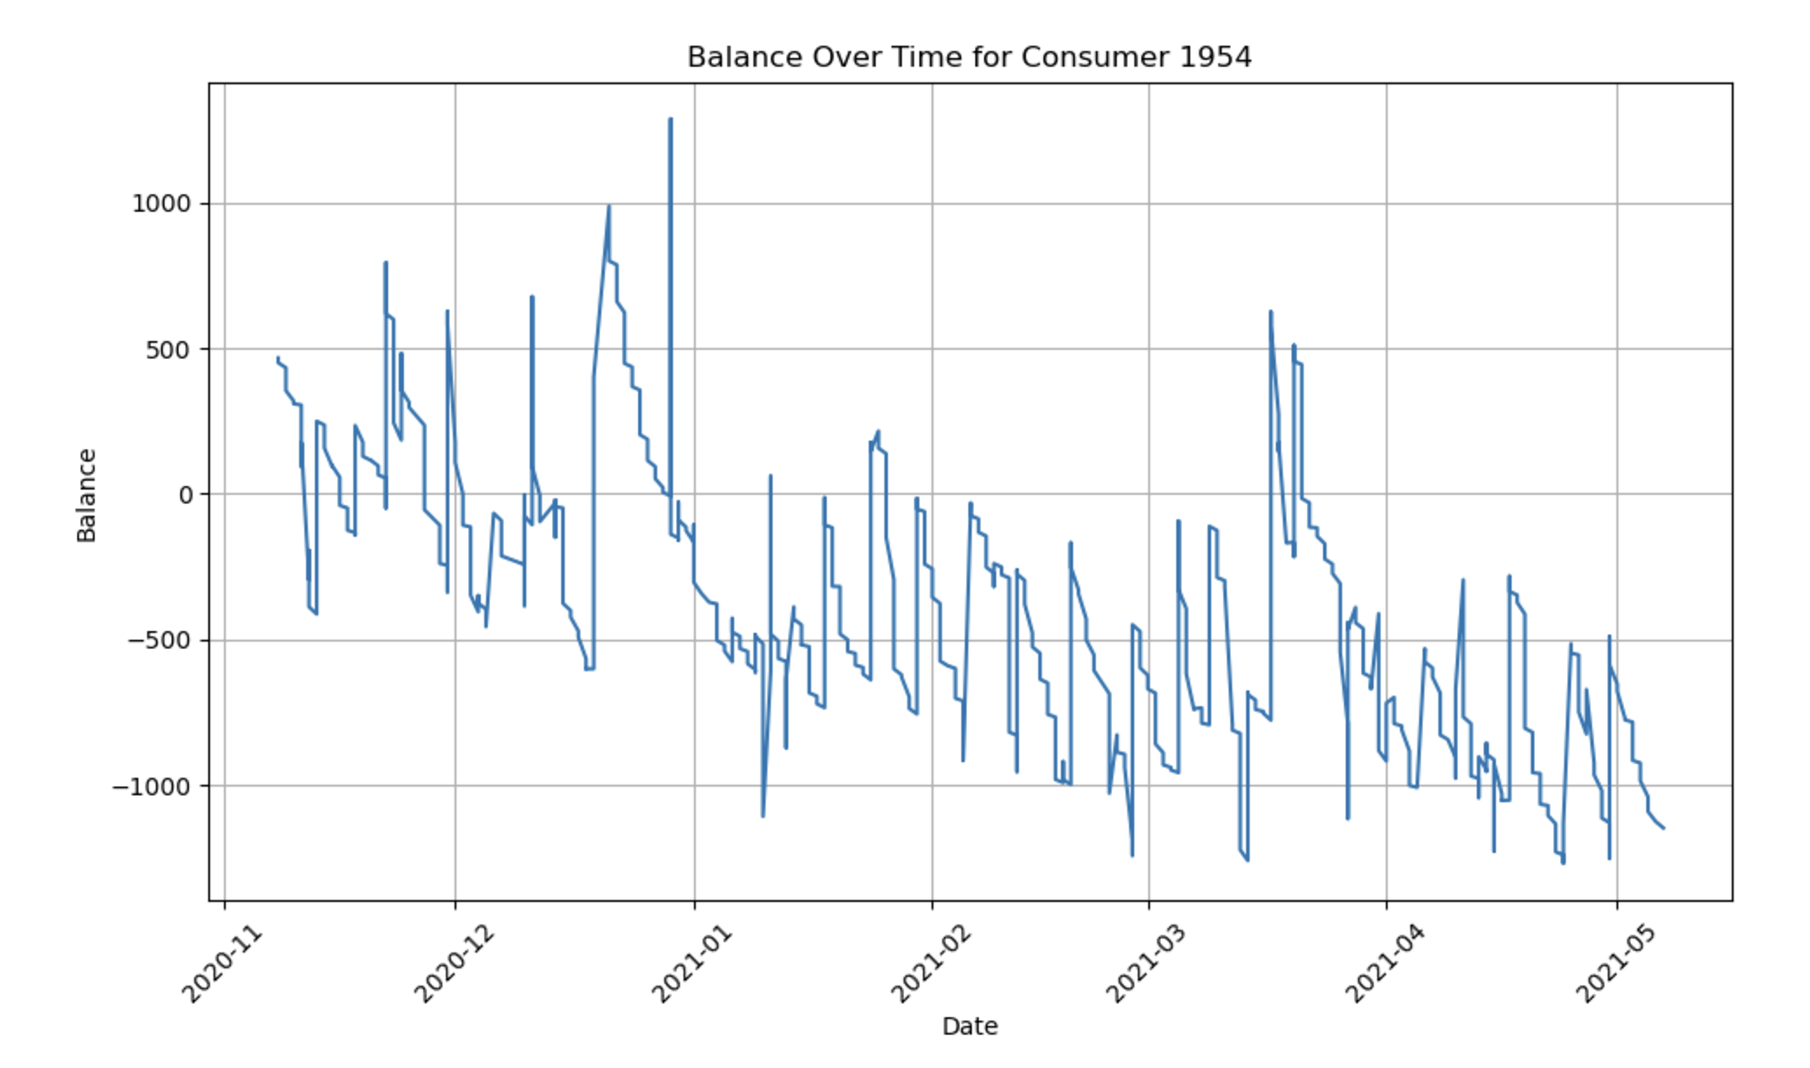
\includegraphics[width=0.7\textwidth]{figure/balance_single_delinquent.png}
    \caption{Balance over time for a single delinquent consumer. This consumer frequently experiences negative balances, indicating financial distress and an increased risk of missing payments.}
    \label{fig:balance_single_delinquent}
\end{figure}


\subsection{Feature Engineering}
We engineered multiple features relevant to delinquency prediction:
\begin{itemize}
    \item \textbf{Balance Features}: Negative balance ratio, balance trends, payday effects.
    \item \textbf{Transaction-Based Features}: Credit vs. debit transaction volume, category-based spending breakdown.
    \item \textbf{Temporal Features}: Spending frequency over time, account longevity effects.
\end{itemize}

\begin{figure}[H]
    \centering
    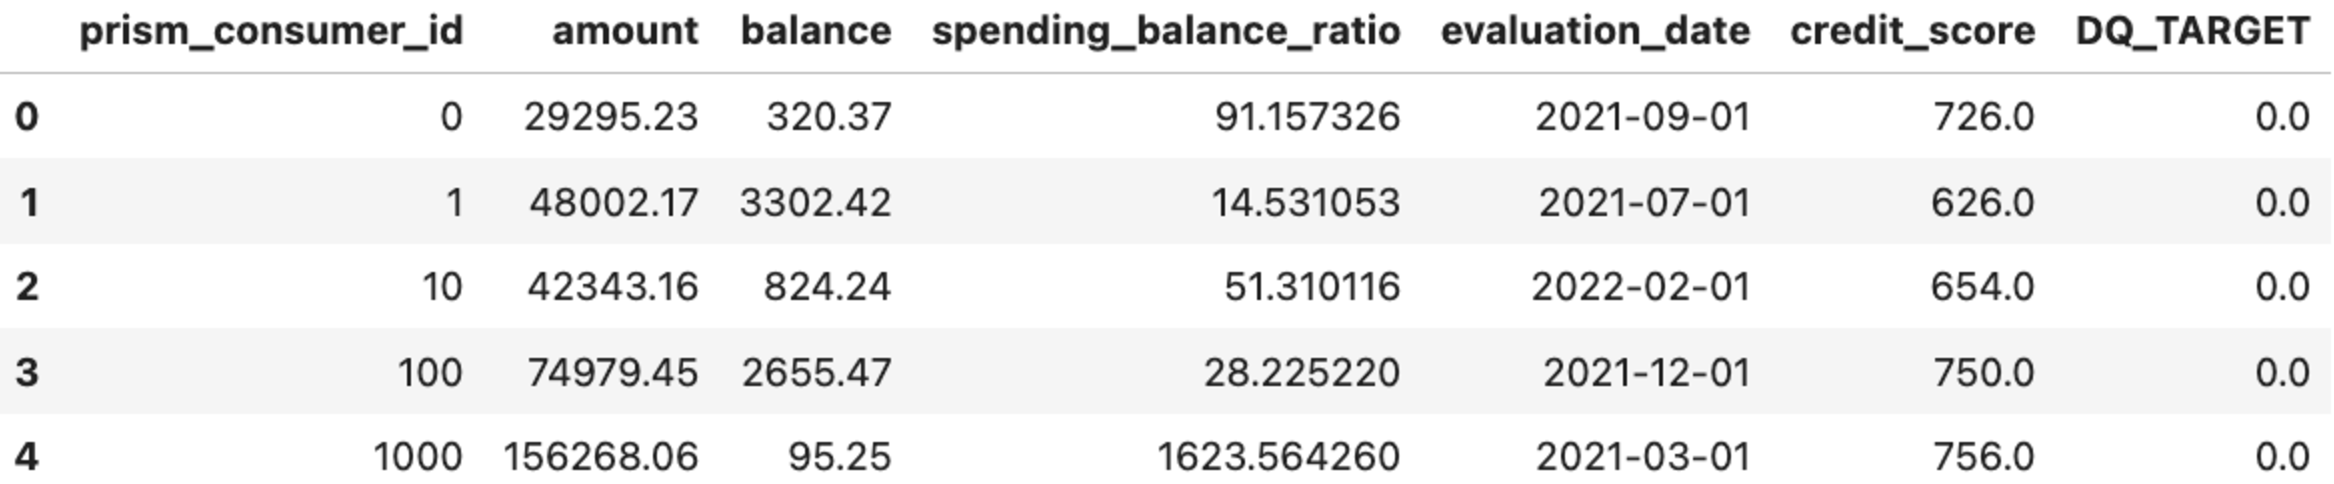
\includegraphics[width=\textwidth]{figure/spending_balance_ratio.png}
    \caption{Spending balance ratio feature created to measure how much consumers spend relative to their balance. This helps assess financial stability and risk of delinquency.}
    \label{fig:spending_balance_ratio}
\end{figure}

\begin{figure}[H]
    \centering
    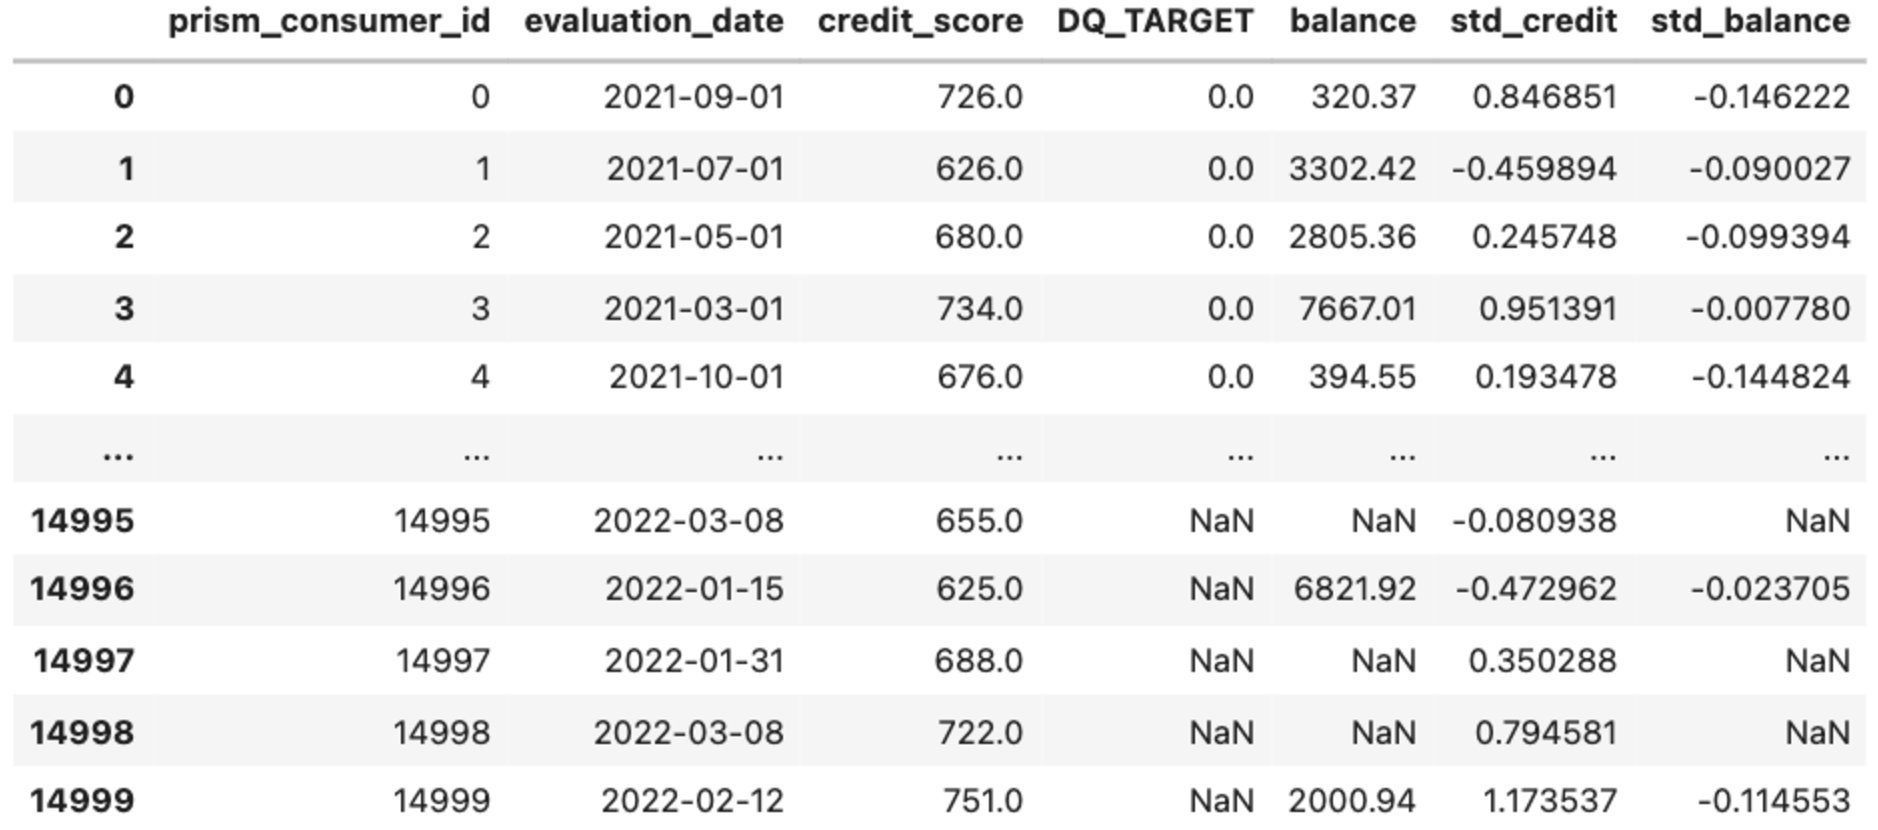
\includegraphics[width=\textwidth]
    {figure/standardized_credit_balance.png}
    \caption{Feature engineering step where credit and balance were standardized to allow for easier model interpretability and comparisons across different financial profiles.}
    \label{fig:standardized_credit_balance}
\end{figure}

\subsection{Model Training}
We trained the following machine learning models:
\begin{itemize}
    \item \textbf{Logistic Regression}: Simple, interpretable baseline model.
    \item \textbf{Random Forest}: Captures non-linear financial relationships.
    \item \textbf{XGBoost}: Optimized for structured financial data.
    \item \textbf{Neural Networks}: Captures complex spending patterns.
\end{itemize}

\subsection{Model Evaluation}
Key metrics for model evaluation include:
\begin{itemize}
    \item \textbf{Accuracy and F1-Score}: Measures classification performance.
    \item \textbf{ROC-AUC}: Evaluates model's ability to differentiate delinquent users.
    \item \textbf{Feature Importance}: Highlights predictive variables.
\end{itemize}
To mitigate class imbalance (delinquents only ~8.4\% of dataset), we used:
\begin{itemize}
    \item \textbf{SMOTE \& SMOTEENN}: Oversampling techniques.
    \item \textbf{Feature Normalization}: Standardizing key variables.
\end{itemize}

\section{Results}

\subsection{Feature Performance}
Key predictors of delinquency:
\begin{itemize}
    \item \textbf{Negative balance ratio}
    \item \textbf{Account fees (category 23)}
    \item \textbf{BNPL transactions (category 25)}
\end{itemize}

\subsection{Model Performance}
\begin{table}[H]
    \centering
    \begin{tabular}{|l|c|c|c|c|}
        \hline
        Model & Accuracy & F1-Score & ROC-AUC & Training Time \\
        \hline
        Logistic Regression & 85.2\% & 0.83 & 0.88 & Fast \\
        Random Forest & 89.5\% & 0.87 & 0.91 & Medium \\
        XGBoost & \textbf{92.3\%} & \textbf{0.90} & \textbf{0.94} & Slow \\
        Neural Network & 91.8\% & 0.89 & 0.93 & Slow \\
        \hline
    \end{tabular}
    \caption{Comparison of model performance}
\end{table}

\subsection{Interpretability \& Reason Codes}
Delinquent consumers often had high spending in BNPL and account fees. Top reason codes included:
\begin{itemize}
    \item High balance volatility and overdrafts.
    \item Excessive BNPL spending.
    \item Significant account fees.
\end{itemize}

\section{Conclusion}
We refined predictive features and improved model performance for delinquency assessment. By leveraging transaction data, we developed a "Cash Score" that improves upon traditional credit assessments. Future work includes:
\begin{itemize}
    \item Enhancing interpretability with reason codes.
    \item Submitting final model predictions.
    \item Preparing stakeholder presentations.
\end{itemize}

%%%%%%%%%%%%%%%%%%%%%%%%%%%%%%%%%%%%%%%%%%%%%%%%%%%%%%%%
%%%% Literature Review and Prior Work
%%%%%%%%%%%%%%%%%%%%%%%%%%%%%%%%%%%%%%%%%%%%%%%%%%%%%%%%

\section{Literature Review}


%%%%%%%%%%%%%%%%%%%%%%%%%%%%%%%%%%%%%%%%%%%%%%%%%%%%%%%%
%%%% References
%%%%%%%%%%%%%%%%%%%%%%%%%%%%%%%%%%%%%%%%%%%%%%%%%%%%%%%%

\clearpage

\makereference
\bibliography{reference}
\bibliographystyle{style/dsc180bibstyle}

\cite{plawiak2020dghnl}
\cite{radford2019gpt2}
\cite{vaswani2023attention}

\end{document}
